\section{Relation between physically based parameters and BSSRDF parametrization}
\label{section:cb_parametrization}
\emph{Artists prefer to define surface albedo and mean multiple scattering distance (characteristic
or visible depth of the SSS). The radiative transport scattering coefficients must therefore be
inferred by inverting the diffusion equation.
Mean-free path gives the scale of the response for a given material. For two materials that differ
only by $l$, we can predict the response of the second material by scaling the response of the first
material by the ratio of their mean-free-paths.}


The Monte Carlo methods of light simulation based on the radiative transport equation use $\sigma_a$
and $\sigma_s$ and $phase function$ as a set parameters defining the optical properties of the SSS
materials \cite{chandrasekhar1960radiative}, \cite{pharr2010physically},
\cite{Jensen:2001:PMS:383259.383319}

Only the case of isotropic phase function is considered in this chapter. Short overview of
anisotropic phase functions can be fount in sections \ref{section:phasefunction} and
\ref{section:phasefunction_approximation}.

On the other side, BSSRDF profile for the Diffusion approximation proposed by Burley and Christensen
\ref{eq:burley} relays on the surface albedo (diffuse surface reflectance) parameter $A$ of the
material:
\[
A = \int\limits_0^\infty R(r)2\pi r dr
\]

In order to maintain consistent parametrization for different SSS integration techniques, the
physically based parameters $\sigma_a$ and $\sigma_s$ have to be mapped to the surface albedo used
by Diffusion Approximation.

The surface albedo $A$, used by in Burley profile, can not be easily analytically computed at
runtime out of $\sigma_a$ and $\sigma_s$. In this work I suggest to find this mapping in advance.
And propose empirical function which fits a wide range of materials.

As an intermediate representation of the physically based parameters I use volumetric scattering
albedo: $\alpha = \sigma_s/\sigma_t = \sigma_s/(\sigma_s + \sigma_a)$. This parametrization is
discussed in the original paper on diffusion approximation proposed by Jensen
\cite{Jensen:2001:PMS:383259.383319}.


The following function is appeared to have a good fit when rendering different materials with
various optical properties:
\begin{equation}
\label{eq:aAMapping}
A(\alpha) = a + b(1- e^{-c\alpha})
\end{equation}
with corresponding constants: $a = 0.0699, b = -3.97\cdot 10^{-05}, c =-10.0$

Using the mapping \ref{eq:aAMapping} it is possible to compute surface albedo $A$ (and consequently
scaling factor $s$) necessary to Christensen-Burley BSSRDF out of volumetric albedo $\alpha$. Which
is directly available from $\sigma_a$ and $\sigma_s$.

\begin{figure}
    \centering
    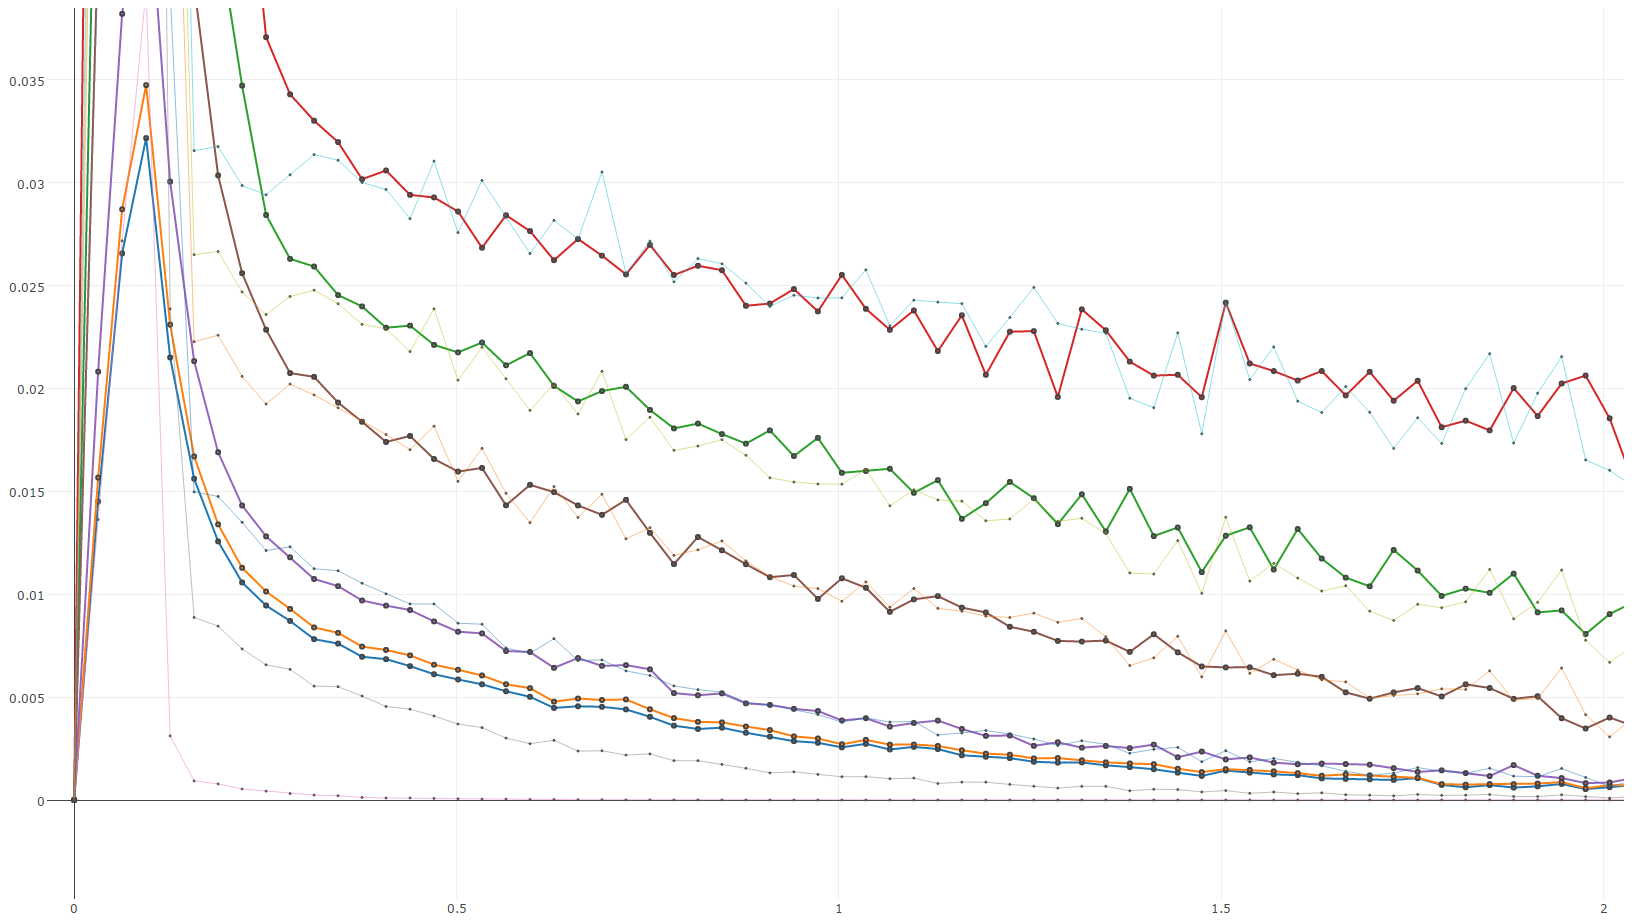
\includegraphics[width=0.98\textwidth]{imgs/plots/aA_fitting}
    \caption{The curve fitting results of the sigmas to albedo}
    \label{fig:albedo_fitting}
\end{figure}
The results of the fitting \ref{eq:aAMapping} are available at figure \ref{fig:albedo_fitting}. The
set of Monte Carlo reference curves are plotted in dashed lines in the corresponding BSSRDF curves
plotted in solid color using the surface albedo computed with the above mentioned fitting function.

As it is seen on the plots, the best fit is possible to achieve for materials with high volumetric
albedo approximately $\alpha>0.67$. But two lowest pairs of curves (green and red with
$\alpha=0.5$ and $\alpha=0.33$ respectively) demonstrate poor match.

This result can be explained by the fundamental limitation of the Diffusion Approximation theory.
Which predict the good approximation for the light transport only in high albedo media. 


The results from the following plot \ref{fig:albedo_fitting} show good match for
Burley profiles (thick lines) to Monte Carlo references (thin lines) for high albedo materials (top
four curves). But there is a significant difference for low albedo materials
with approximately $A<0.3$

Note that two lower thick lines does not not correspond to lower two thin lines.
And this result is consistent with the assumptions of the diffusion theory of
the light transport in participating media.